%\chapter{Predicting Profitability Using Machine Learning}
\chapter{Directional Profitability Predictions with Random Forests} \label{Chapter:ABIS}

\section{Introduction}
\blfootnote{
This chapter contains material from the following working paper: Vic Anand, Robert Brunner, Kelechi Ikegwu, and Theodore Sougiannis. Predicting profitability using machine learning. SSRN, Oct 2019. URL \url{https://papers.ssrn.com/sol3/papers.cfm?abstract_id= 3466478 }

	%\nobibliography{thesisbib}
	%\begin{itemize}
	%	\item\bibentry{ABIS}
	%\end{itemize}
	
}


%\RC{This first statement should be clarified. Not all countries/people would agree.}
% Not the goal but a goal.  In  a socialist society, everyone has same amount of wealth ideally.  Why wouldn't they want to maxmize wealth of economic overall?

An economic goal of a society is to maximize wealth.  In order to maximize wealth, resources such as labor, capital, and natural resources must be allocated efficiently to firms. Capital markets (such as the stock market) allow capital to be efficiently allocated to said firms. Firm profitability can affect society, whether through job growth or loss, the offered services, the provision of goods, or personal gain or loss (see \cite{IntAccBook}).  Predicting the future profitability for firms is an essential endeavor as it is central to the valuation of the firm and the securities they issue (see \cite{Monahan}). 

A study by \cite{Bradshaw} provides evidence that analysts' predictions are not superior to random walk predictions, indicating that traditional methods provide little efficacy. \cite{Monahan} conducts a review and discussion on the accounting research related to out-of-sample profitability predictions.  He provides evidence that models in prior works have lower out-of-sample accuracy than random walk models. This provides motivation to seek an alternative method, given the shortcomings of traditional methods.   \cite{ABIS:ML:EX1},  \cite{ABIS:ML:EX2},  \cite{ABIS:ML:EX3},  and \cite{ABIS:ML:EX4} are relatively recent examples that demonstrate the effectiveness of machine learning for prediction and inference in a variety of applications.  Thus, we explore machine learning methods to predict the future profitability of firms.
 
An approach outlined in \cite{Monahan} is to select five items: the labels (or what to predict), the features (or predictors), a regression model (where the functional form is determined by the researcher),  and the training and testing datasets.  One can use a parametric approach and assume the functional form of \(f\) (see Equation \ref{eq:function}) and estimate a set parameters; however,  it is likely that the functional form will not match the true unknown form of \(f\) which would provide poor results.  Given our objective to find the best \(f\) in Equation \ref{eq:function} that predicts \(Y\) reasonably well, we use non-parametric methods.  In addition, we employ cross-validation, described in section \ref{sec:validationApproach}, to avoid overfitting the model.  Lastly, we use machine learning to predict directional changes rather than the magnitude of changes in the firm's profitability. We make this choice to account for working with a smaller dataset.  \cite{BB68} and \cite{OU1989295} have shown that the future directional change of profitability is a useful indicator. 

Our stated research objective is to determine if a machine learning model can be constructed to outperform a random walk model.  This chapter will describe the datasets used in this study and the methods used to predict firms' directional change of profitability.  Finally, comparative analyses will be conducted between the proposed model and random walk model, followed by a discussion of results and potential future directions of this research.

\section{Data} \label{sec:ABIS:Data}

We follow the data selection process described in \cite{HOU2012504} in this research. We use all observations from the fiscal years 1963 - 2016 from the Compustat fundamentals annual file. We merge this data set with the CRSP monthly returns file, which includes all securities listed on the NYSE,  Amex,  and Nasdaq markets. The securities selected have share codes 10 or 11, indicating that they are ordinary common shares of US companies and exclude ADR's and REITs. We remove observations if total assets, common equity, dividends, income before extraordinary items,  or accruals are missing, resulting in 194,172 observations.  Given the objective to predict the future direction of profitability for firms, each firm must have at least three observations; the rationale behind this choice is to compute two price changes for a firm. Excluding firms with fewer than four years of observations, the final dataset consists of 160,653 observations.  

While we have 160,653 observations in our dataset the firm observations are significantly smaller. For example, in Figure \ref{fig:ABIS-DATA} we see the annual return on equity for firms in our sample. Some firms, such as International Paper, have a long history of reported profitability. However, most firms in our sample do not have a long history. For example, in Figure \ref{fig:ABIS-DATA} Smiths Transfer Corp Staunton Va was acquired by another firm and stopped reporting earnings. A W Computer Systems Inc ceased operations and liquidated its assets. Figure \ref{fig:FirmObs} shows the distribution of firm observations in our sample. We can observe that there are more firms with a short history than firms with a long history. This  observation influenced our decision to predict directional changes for initial research.

The following variables were retrieved and computed for this research: Return on common equity (ROE),  Return on assets (ROA), return on net operating assets (RNOA), Cash flow from operations (CFO),  and free cash flow (FCF).  Tables \ref{tab:CompustatVariables} and \ref{tab:ComputstatCompute} contains more details about the variables used from Compustat and Table \ref{tab:ProfitMeasures} shows how the profitability measures are computed.   



%ROE, ROA, RNOA, CFO, and FCF are selected as the labels for separate machine learning models.   To state this differently a machine learning model will use a features to predict  the change in ROE, ROA, RNOA, CFO, or FCF.  Year to year change is computed with each of the labels where +1 represents increase, -1 represents decrease, and 0 represents no change in the profitability measure.  Table \ref{} shows the percentage of profitability measures that increase, decrease, or have no change from year to year. 

Table \ref{tab:CompustatDescribe} provides descriptive statistics on variables retrieved from Compustat. Outliers are present in most variables, and all of them have positively skewed distributions given that the mean is greater than the median. Table \ref{tab:ProfitDescribe} provides the descriptive statistics on profitability measures.  Since the raw variables construct the profitability measures, their values are also extreme.  However, unlike the raw variables, the distributions of the targets are negatively skewed (the mean is smaller than the median).  Table \ref{tab:TargetPercentIncreases} shows the percentage of times the target variables increase in the holdout period or testing data (2012-2015).   With the exception of CFO and FCF during 2013,  there are no relatively significant class imbalances for directional changes in profitability measures. 

Tables \ref{tab:ROECorr},  \ref{tab:ROACorr},  \ref{tab:RNOACorr},  \ref{tab:FCFCorr}, and \ref{tab:CFOCorr} show the Pearson correlations between variables that will serve as the features in the random forest models.  Each table shows the correlations between the profitability measure, the mean industry profitability measure, the median industry profitability measure, the standard deviation of the industry profitability measure,  and the profitability measure at time \(t-1\),  and \(t-2\).  We note that we can incorporate additional features that can increase the performance of our models; however, as an initial step we examine whether we can outperform the random walk with a minimal feature set.  Since correlations of raw variables are extreme due to large outliers, we truncate each variable at 2.5\% on each side of its distribution.  Many of the features in these tables are correlated. Nevertheless, the proposed machine learning method performance is insensitive to multicollinearity.   %Table \ref{tab:AutCorrProfitability} shows the autocorrelations of truncated profitability features.  With the exception of CFO, the second-order autocorrelations are marginally smaller than the first-order autocorrelations for all profitability measures. 

\section{Methods}

\subsection{Cross Validation for Time Series} \label{sec:CV-TS}

For this work, the supervised learning paradigm described in section \ref{sec:SupervisedLearning} will be employed.  We use 90\% of the data for training and the remaining 10\% for testing. The first 90\% of data contains data from the fiscal years 1963-2011, and the last 10\% of data is from 2011-2016.  Given the objective to predict the year-to-year change, we cannot predict using features for firms in the fiscal year 2016 because the fiscal year 2017 is not in the sample. Given the time-series nature of the data, we use blocked \(k\)-fold cross-validation as described in \cite{cerqueira2019evaluating}. The difference between blocked \(k\)-fold cross-validation and \(k\)-fold cross-validation is that the observations are not randomly shuffled and then divided into k folds. Instead, the observations are split into \(k\) blocks of contiguous observations. 

%The natural order of observations is preserved within blocks but not across them. A machine learning model will learn to predict year to year price change for a particular profitability measure. For the first iteration blocked \(k\)- fold cross validation the model will have access to features from the \(1^{st}\) block of observations in the data set and predict how the profitability measure will change for the \(2^{nd}\) block of data  . For the \(2^{nd}\) iteration the model will have access to features from the  \(1^{st}\) and \(2^{nd}\)  chunks of data to predict how the profitability measure will change for the next chunk.  This process will repeat  \(k-1\) times (see Figure \ref{} for a detailed explanation).

\subsection{Tree based Machine Learning Methods}

%There are many models that can be used within the realm of machine learning to predict the profitability of price change.  
Many machine learning models can provide high accuracy scores. However, there is a trade-off between interoperability and performance (see  \cite{ISL}, Chapter 2).  Given that the research objective is more aligned with prediction than inference, we emphasize model performance. Tree-based models are flexible, simple to implement, and have high performance (see \cite{ISL},  Chapter 8). In addition to this, tree-based methods can handle multicollinearity and non-linearity better than linear regression methods traditionally used in the financial accounting domain (see \cite{Monahan}).  

\subsection{Decision Trees} \label{sec:DecisionTrees}

Decision Trees are the building blocks of tree-based machine learning methods.  Decision Trees are directed graphs with no cycles, meaning there are no nodes with edges to the same node, there is no more than one edge connecting two nodes, and there is only one path connecting two nodes.  We refer to edges in trees as branches.  Consider three nodes node \(A\),  \(B\), and \(C\), if node \(A\) has a branch to nodes \(B\) and \(C\),  \(B\) and \(C\) are the children of node \(A\). In this case, node \(A\) is the parent of nodes \(B\) and \(C\).  The root node starts the decision tree and does not have a parent.  Lastly, a node with no children signifies a stopping point  within the decision tree and is referred to as a leaf node (see Figure \ref{fig:DecisionTree} for an example).

In a supervised machine learning paradigm, decision trees are constructed from the training data set.  Each node in the decision tree will represent the training features (or feature space, i.e. \(X_1,...,X_p\)) partitioned into particular regions. Using the CART algorithm (see \cite{CART}) a decision tree will create \(m\) distinct non-overlapping regions \(R\). The root node will contain a rule to partition the feature space into two non-overlapping regions (\(R_1\) and \(R_2\)). The process will repeat recursively, in other words, both \(R_1\) and \(R2\) will be further divided by a splitting criteria to partition the data into two additional regions. \(R1\) will be divided into \(R_3\) and \(R_4\)  and \(R_2\) into  \(R_5\) and \(R_6\). 

%  A common criteria is to determine which feature that has the largest amount of certainty (or smallest amount of entropy).

In a classification setting, a decision tree at a given region will determine the most optimal feature to select from the set of features to partition the data.  The selection is typically based on the feature's ability to minimize error.  A common metric is gini-impurity, where gini-impurity measures the variance across \(C\) classes. We can define gini-impurity as: 

\begin{equation}
\label{eq:GiniImpurity}
G_{index} = \sum_{i=1}^{C} p(i) \cdot (i - p(i))
\end{equation}

\noindent where \(C\) is the number of classes in a label and \(p(i)\) is the probability of an observation labeled class \(i\).  A small value of gini-impurity indicates that a particular region has many observations from a single class. 

Decision trees have stopping criteria.  For example, we stop creating additional regions when a child has less than a defined number of observations at a particular region or when the difference of gini-impurity between the parent and its children is less than a specified amount.  Lastly, to predict values of \(Y\) from another set of data (containing the same features), new observations can be passed into the trained tree.  The trained tree will select the appropriate region for an observation based on the splitting criteria rules. 

Decision Trees offer an intuitive explanation of the results it produces. However, there are some caveats to this method.  A few additional observations or any modification to observations in a feature space can drastically change a decision tree because it is using a greedy search to build a tree (see \cite{koning2017decision}). Meaning that at each stage of the tree-building process, a node is split using a local optimal choice instead of a choice that will find the optimal choice on a global level. 

\subsection{Random Forests} \label{sec:RandomForest}

Random forests can overcome some of the shortcomings of decision trees.  Random forests are an ensemble of decision trees used to make predictions. However, a random forest is less interpretable than a single decision tree.  A random forest will create \(B\) decision trees.  For each decision tree,  the random forest will assign a random dataset to each decision tree in the forest by sampling the data with replacement (or bootstrapping). In addition to this, the random forest will choose a subset of random features (with replacement) to construct each decision tree. 
 
The rationale behind selecting only a subset of features is to decorrelate trees, meaning that if a feature is important, it will not always be used as a top-level split thereby producing unique decision trees. Each tree is built and predictions made by using the random data and features in the method outlined in the Decision Trees subsection at \ref{sec:DecisionTrees}. To make predictions in a classification setting \(B\), decision trees will make a prediction using the features from the bootstrapped data. The most common prediction class is used as the prediction for the forest of trees (which is referred to as the majority vote).

%\section{Implementation to Predict Directional Profitability}
%\section{Random Forest Directional Profitability Prediction }

\section{Random Forest Implementation to Predict Directional Profitability}

For this research, annual profitability changes (ROE, ROA, RNOA, CFO, and FCF) are coded as +1 for an increase and -1 for a decrease for individual firms in the dataset described in section \ref{sec:ABIS:Data}. The features used are described in section \ref{sec:CAnalyses}. With data sorted by fiscal year, for a change in a specific profitability measure that feature set (see Tables \ref{tab:ROECorr},  \ref{tab:ROACorr},  \ref{tab:RNOACorr},  \ref{tab:FCFCorr}, and \ref{tab:CFOCorr}) will be partitioned into training and testing sets. The first 90\% of observations (fiscal years between 1963-2011) are used to train and build \(B\) trees.  The remaining 10\% of observations (2012-2015) are used to make predictions out of sample. 

While building \(B\) decision trees,  cross-validation, as described in \ref{sec:CV-TS}, is employed. The training data will have \(k\) folds (where \(k=5\)) grouped by fiscal year.  Each particular fold will consist of observations for particular firm-years.  Each decision tree in the forest will bootstrap from each fold and select random features. The decision tree will then train and build a tree based on the methodology outlined in \ref{sec:DecisionTrees}. The random forest of trees will make predictions on the validation sets with the process outlined in section \ref{sec:RandomForest}. Finally, the trained random forest will  make predictions out-of-sample on observations from the test set.

\section{Random Walk Benchmark Models} \label{sec:RWModel}

The random walk is a model of a stochastic process.  \cite{Campbell1997} (hereafter CLM)  described it by the following equation: 

\begin{equation}
\label{eq:RW1}
P_t = \mu + P_{t-1} + \epsilon_t 
\end{equation}

\noindent In Equation \ref{eq:RW1}, \(P_t\) is the value of some state variable at time \(t, \mu\) is a drift term that we will assume is 0, and \(\epsilon_t\) is a disturbance, or increment.  CLM note that a common assumption is that the disturbance term is independent and identically distributed, with mean zero and variance \(\sigma^2\),  i.e.  \( \epsilon_t \sim IID(o,\sigma^2)\). 

The random walk is a mathematical description of a process, not a forecasting tool. However, some papers (i.e.  \cite{Bradshaw}) that wish to use the random walk as a benchmark for their results treat it as a forecasting tool by taking the expected value of both sides of Equation  \ref{eq:RW1}. That yields the following:

\begin{equation}
\label{eq:RW2}
E[P_{t+1}] = P_t \Leftrightarrow E[P_{t+1} - P_t] = 0
\end{equation}

\noindent These papers reason that since the expected value of \(P_{t+1}\) is \(P_t\), the best forecast of \(P_{t+1}\) is also \(P_t\). However, the random walk does not actually predict \(P_{t+1}\). It simply states that the expected magnitude of change in \(P\) at any time is zero. In other words, if you observe changes in \(P\) over a long time series, the average change will be zero.

To be consistent with prior literature, we treat the random walk model as a forecasting tool. However, our work introduces a complication. Prior literature forecasts the magnitude of some variable. By contrast, we forecast the direction of change in our variables. Applying the random walk to our setting, therefore, requires some additional steps. CLM notes that the expected value of \(\epsilon_t\) is zero, but without additional assumptions, we cannot know the proportion of increases and decreases in \(\epsilon_t\).

\subsection{Random Walk: Benchmark 1}

Rearranging Equation \ref{eq:RW1} and setting the drift term to zero yields \(P_t - P_{t-1} = \epsilon_t\). Thus, the change in profitability is exactly equal to the disturbance term. That implies that the sign of the change in profitability is equal to the sign of the disturbance term. By assumption,  \(\epsilon_t \sim IID(0,\sigma^2)\), and CLM (p.32) state that “perhaps the most common distributional assumption for the innovations or increments \(\epsilon_t\) is normality.” Normality implies a 50-50 chance of an up or down movement since the normal distribution is symmetric. Therefore, our first random walk prediction should be that profitability is equally likely to increase or decrease.

Under the assumption that the error term is equally likely to increase or decrease, we find that the random walk model has an expected accuracy of 50\%. To see this, assume the testing subsample contains \(N\) observations, and  \(0 \leq p \leq 1\) is the fraction of increases. Then \(p\) of those observations increases, and \((1-p)N\) decreases. For any observation, the random walk will predict an increase 50\% of the time and a decrease 50\% of the time. Thus, of the \(p\) increases, on average 0.5\(pN\) will be classified accurately.  Similarly, of the \((1-p)N\) decreases, \(0.5(1-p)N\) will be classified accurately.  For the overall sample, the fraction that will be accurately classified is:

\[Accuracy= \frac{0.5pN+0.5(1-p)N}{pN+(1-p)N}=\frac{1}{2}\]

\noindent Note that the classification accuracy of this interpretation of the random walk is invariant to the fraction of increases in the data. For any value of \(p\), if we assume increases and decreases are equally likely, this random walk model will accurately predict on average the outcome 50\% of the time.

\subsection{Random Walk: Non-normal Error Term}

The random walk model requires that the error term has zero mean and finite variance, \(\epsilon_t \sim I(0,\sigma^2)\). This restriction does not imply normality of the error term: \(\epsilon_t\) could have any arbitrary probability of increase as long as its expected value is zero.  For example,  if \(\frac{2}{3}\) of the time \(\epsilon_t\) increases by 1, and \(\frac{1}{3}\) of the time it decreases by 2,  it has mean zero.  A distributional assumption other than normality may be appropriate if the actual fraction of increases in the data is not 50\%.

%\cite{ABIS} shows in Appendix B that if the fraction of increases in \(\epsilon_t\) is within the range of 40 – 60\%, then the classification accuracy of a non-normal random walk model remains close to 50\%.  
\cite{ABIS} showed in Appendix B  that even if we assume \(\epsilon_t\) will increase 40\%-60\% of the time, the classification accuracy ranges from 48\%-52\% which is very close to the 50\% by assuming a normally distributed error term. Table \ref{tab:TargetPercentIncreases} shows that,  for most measures in most years, the actual fraction of increases in our sample are very close to 50\%. Even in the most extreme case (in 2013,  CFO and FCF increase 43.3\% and 42.5\% of the time).

\subsection{Random Walk: Benchmark 2}

As an alternative interpretation of applying the random walk model to forecasting, consider the following equations:

\begin{align}
	P_t &= P_{t-1} + \epsilon \label{eq:RW3}\\
	P_{t-1} &= P_{t-2} + \epsilon_{t-1} \label{eq:RW4}
\end{align}

\noindent Subtracting Equation \ref{eq:RW4} from Equation \ref{eq:RW3} yields:

\begin{align}
(P_t - P_{t-1}) = (P_{t-1} - P_{t-2}) + (\epsilon_t - \epsilon_{t-1}) \nonumber \\
\Delta P_t = \Delta P_{t-1} + (\epsilon_t - \epsilon_{t-1}) \label{eq:RW5}
\end{align}

If we take the expected value of both sides,  Equation \ref{eq:RW5} reduces to  \(\Delta P_t = \Delta P_{t-1}\) since, by assumption, \(E[\epsilon_t] = 0, \forall t \). Under this interpretation, in expectation, an increase in a profitability measure in period \(t-1\) will persist into period \(t\). Thus, our second random walk prediction is that the sign of the change in a measure in one period will persist into the subsequent period.


\section{Comparative Analyses} \label{sec:CAnalyses}

To answer the research objective,  we conduct comparative analyses between the benchmark random walk models (described in \ref{sec:RWModel}) and the random forest models (described in \ref{sec:RandomForest}). We employ multiple random forests to predict specific profitability measures and add additional features to each random forest for each subsequent analysis. These analyses provide insight as to whether specific features are informative and yield more accurate estimates.

We perform the analyses in two phases.  In the first phase,  we test whether Random Forests performs better with winsorized or unwinsorized data \footnote{See \cite{winsor} for a detailed explanation and review of winsorization.}.  In the second phase, we employ multiple random forests to learn the incremental value of additional variables used in fundamental analysis. 

%\RC{Do you think you should define winsorization?}

\subsection{Phase 1: Effect of Winsorization}

The purpose of phase 1 is to test the effect of winsorization on predictive accuracy.  Our prior is that winsorization will not affect the predictive accuracy of random forests.  In phase 1, we use a minimal information set in which each firm-year observation consists of the firm identifier (PERMNO), fiscal year, the contemporaneous value of a measure (i.e., ROE), and the label or change that occurs in the subsequent year (i.e., increase or decrease). We create three random forests for this phase.  We train the first random forest on un-winsorized data and refer to this as analysis 1-1.  For analysis 1-2, we train the second random forest on data where the measure is winsorized at 1\% on each side. For analysis 1-3 we repeat the same methodology as analysis 1-2 where the measure is winsorized at 2.5\% on each side.

\subsection{Phase 2: Effect of Adding Additional Fundamental Information}
In phase 2, we progressively add information about each firm's industry.  We begin with analysis 2-1, and add SIC codes as a feature.  Analysis 2-2 adds industry information to the feature set.  For each firm-year observation in analysis 2-2 we add the industry mean, median, and standard deviation for the measure. For example, consider predicting the change in annual RNOA for IBM during the fiscal year 2000.  The industry mean, median, and standard deviation of RNOA for IBM's Industry are used as features during the year 2000.  The firm's 4-digit SIC code determines the industry.

Analysis 2-3 repeats analysis 2-2 while including the lag of the profitability measure.  For example, if the measure is ROE, then for IBM in the year 2000 its ROE from 1999 is included as a feature in addition to other features from analysis 2-2.  For the final analysis 2-4,  we repeat analysis 2-3 while including the 2nd lag of the profitability measure.  Following the IBM example for analysis 2-3, its ROE from 1998 is included as a feature.

\section{Results}

\subsection{Phase 1 Results and Discussion}
Phase 1 tests the predictive power of random forests with minimal information. It also tests the effect of winsorizing the input data, a common practice in accounting research.  In phase 1, we create three random forests per profitability measure and use a minimal set of features. For each random forest, the only predictors (features) in each observation are a firm identifier (PERMNO),  fiscal year, and the contemporaneous value of the profitability measure. The label is a categorical variable that indicates whether profitability increased or decreased in the subsequent year. The input data's non-categorical measures are winsorized at three levels, 0\%, 1\%, and 2.5\% on each side. Analysis 1-1 uses a random forest to make predictions on the non-winsorized data, 1-2 uses the 1\% winsorized data, and 1-3 uses the 2.5\% winsorized data.

We begin with the default values for model parameters in sci-kit learn version 0.22 (see \cite{scikit-learn}). We varied the number of trees used in a forest for each measure to predict the change in profitability. We found for all measures that there was no significant improvement in performance after using 30 decision trees in a random forest, see Figure \ref{fig:ValidationCurve-A1-Trees}. In Figure \ref{fig:ValidationCurve-A1-Trees}, all subplots share the same x-axis, which represents the number of trees used in a forest. The y-axis for each subplot represents the accuracy score for a particular measure.

In each subplot, the dashed line with the circle markers represents the mean training scores during cross-validation. The shaded region surrounding the dashed line with circle markers represents the variance of the training accuracy scores during cross-validation.  This shaded region is not visible because the variance of the \(k-1\) training scores is very small. The solid line with star markers represents the mean cross-validation accuracy score, and the shaded-in region represents the variance of the cross-validation scores for each fold.

Given the large gap between the mean training and cross-validation accuracy scores, it is probable that the random forests are over-fitting the data. With the current model parameters (while varying the number of trees used in the random forest), the model is learning information from the training data that is noise. The current parameters impede the model's ability to generalize to the cross-validation data well. To decrease the model's variance (or flexibility), we vary the depth of each decision tree in the forest. 

Figure \ref{fig:ValidationCurve-A1-Depth} shows the mean training and cross-validation scores for a random forest with 30 trees as the maximum depth is varied.  As the depth increases, the model becomes more flexible. Across all profitability measures, one can see that the model can learn from the training data fairly well with high training accuracy scores. However, the highly flexible models cannot generalize well to the cross-validation data and perform worst than other models with a smaller maximum depth. Thus, we select the maximum depth that yields a model with relatively low variance and bias for each profitability measure. We forgo displaying similar plots for analyses 1-2 and 1-3 because the effect and accuracy scores are similar. 

Table \ref{tab:MaxDepthA1} shows the model maximum depth selected for analyses 1-1, 1-2, and 1-3. Tables \ref{tab:ROE-1},  \ref{tab:ROA-1}, \ref{tab:RNOA-1}, \ref{tab:CFO-1}, and \ref{tab:FCF-1} show the mean training, mean cross-validation, and testing scores for the ROE, ROA, RNOA, CFO, and FCF measures respectively. In addition to showing the cross-validation scores, we show the random walk model performance on the data,  and the feature importance of each variable. 

The results show that the random forest can outperform the random walk models for each measure in predicting the change of profitability with a minimum set of features. In addition to this, when excluding the ROE measure we find no significant difference in mean testing accuracies between winsorized and non-winsorized data. Analysis 1-1 (no winsorization) and 1-3 (2.5\% per side winsorization) had a mean test accuracy of 55.2\%; however, analysis 1-2 (1\% per side winsorization) had a mean test accuracy of 56.8\%. The remaining analyses for the other profitability measures have mean testing accuracies within 1\% of each other. These results provide evidence that winsorization has a negligible effect on performance out of sample.

To summarize,  traditional approaches have struggled in the past to out-perform a random walk model. With a minimum amount of features (company identifier, profitability measure, and fiscal year), we find that a random forest model is able to out-perform a random walk model in predicting annual profitability changes. In addition, we find that winsorizing the data (which is a traditional method used to handle outliers in financial accounting) has a negligible effect on the performance of a random forest model.

\subsection{Phase 2 Results and Discussion}

Given that there is no significant effect of winsorization on the random forest model's performance, we forgo using the winsorized datasets. We create additional random forests where each successive forest incrementally adds features. In analysis 2-1, we include the firm's industry as a feature. Analysis 2-2 includes descriptive statistics about the firm's industry at a given year. The specific statistics used are mean, median, and standard deviation. Analysis 2-3 adds the previous lag value of the profitability measure (i.e., the profitability measure at \(t-1\)), and analysis 2-4 includes the two previous lag values of the profitability measure (i.e., \(t-1, t-2\)). Tables \ref{tab:ROE-2}, \ref{tab:ROA-2}, \ref{tab:RNOA-2}, \ref{tab:CFO-2}, and \ref{tab:FCF-2} report the results from the second set of analyses. 

Similar to the first set of analyses, all random forest models outperform the random walk models. Comparing the second set of analyses to analysis 1-1 (non-winsorized data with a minimum set of features), we find mixed results for each profitability measure. For CFO and FCF, we find improvements across all sets of analyses. However, for ROE, ROA, and RNOA there is little to no improvement from analysis 1-1.  We find that CFO and FCF random forest models utilize the feature \(CFO_t\) and \(FCF_t\) the most throughout all analyses. This finding provides evidence that the best feature to predict the future directional change of a measure is the current value of the measure for CFO and FCF. 

The RNOA, ROA, and ROE analyses still utilize \(RNOA_t\), \(ROA_t\), and \(ROE_t\) respectively more than any other feature; however, they utilize it significantly less than the random forest models that predict CFO and FCF. For example, in analysis 2-3  for RNOA, ROA, ROE, CFO, and FCF the previous lagged measures are the second most used by the model. The feature importance of CFO and FCF are 69.2\% and 78.5\% more than the lagged value (\(CFO_{t-1}\) and \(FCF_{t-1}\)). However, the ROE, ROA, and RNOA measures use their respective current values at \(t\) 45.7\%, 50.3\%, and 45.8\% more than the lagged values. In addition to this, we find that ROE's performance improves more than ROA and RNOA. This finding further provides evidence that the most information about future profitability changes is in the profitability measure's current value.

\section{Conclusion and Future Work}

In this chapter, we explored the utility of random forest trees in a supervised learning paradigm to predict the annual direction of profitability for firms with minimal information. This study's motivation stems from the fact that the accounting literature shows that traditional regression methods cannot produce models superior to random walk models when predicting out of sample. We also explore the advantages of following a supervised learning paradigm to predict directional change. For example, random forests are insensitive to multicollinearity, and properly utilizing the supervised paradigm discovers a functional form that generalizes well to new data.

We implement and train random forests in a classification setting using a large sample of US firms over the period 1963-2011.  We generate out-of-sample predictions of directional changes (increases or decreases) in five profitability measures: return on equity (ROE), return on assets (ROA), return on net operating assets (RNOA), cash flow from operations (CFO), and free cash flow (FCF) from 2011-2016. We found that the classification accuracy for each measure outperformed the random walk models.  The accuracy does not tend to decline with a four-year forecast horizon significantly for the out of sample predictions. In addition to these findings, models with a strong reliance on a profitability measure's current value provided more accurate estimates of the future directional change in profitability.   The results also show that the random forest does not find the accrual profitability measures (ROE,  ROA,  and RNOA) at the year \(t\) as useful as the cash flow measures (CFO and FCF) in predicting the future.

We can improve these results further by selecting a model that yields better performance but offers less interpretability. Given that we focus on a minimal set of features in this research, we can incorporate additional features for additional performance gains. Utilizing more data, we can extend the methodology outlined in this paper to a regression setting and make predictions about the magnitudes of profitability. 


The results shown in the paper are promising since  we outperform a random walk model for all of the profitability measures used in this study. The methods used in this chapter are robust to econometric issues such as multicollinearity and outliers.  When used correctly, the methodology outlined in this paper can produce models that generalize well to out of sample data.  Machine learning has simplified and solved problems in many aspects of our lives.  The results show the benefit that it can have on predicting the profitability of firms in a financial accounting research setting.

\clearpage

\section{Figures and Tables}

%\begin{minipage}{0.8\textheight}
   %\centerline{ \includegraphics[width=0.85\textwidth, keepaspectratio]{figures/ABIS/analysis_1-1_ValidationCurveTrees.png}}
    %\captionof{figure}{This figure shows validation curves for each measure in Analysis 1-1 varying the amount of trees. }
%    \label{fig:ValidationCurve-A1-Trees}
%\end{minipage}

\begin{figure*}[!htb]
    \centering
      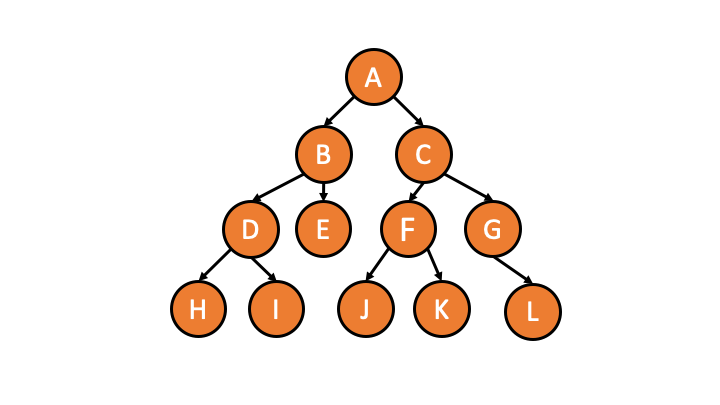
\includegraphics[width=\textwidth]{figures/ppt/DecisionTree.png}

    \caption{
	This figure shows an example of a Decision Tree. This is essentially a graph with no cycles.  Each circle represents a node (the label of the node is a letter inside of the node) and the arrows represent directional edges (branches) to another node. Node \(A\) is the root node of this tree and is where the decision tree begins. Potential outcomes from the root node lead to different states that are represented in nodes \(B\) and \(C\). \(B\) and \(C\) are the children of \(A\).  Nodes \(B\) and \(C\) have children and their children has children. Nodes \(H, I, E, J, K,\) and \(L\) are the leaf nodes of this tree because they have no children.
     }
      \label{fig:DecisionTree}
  \end{figure*}

\begin{sidewaysfigure*}[htb!]
    \centering
    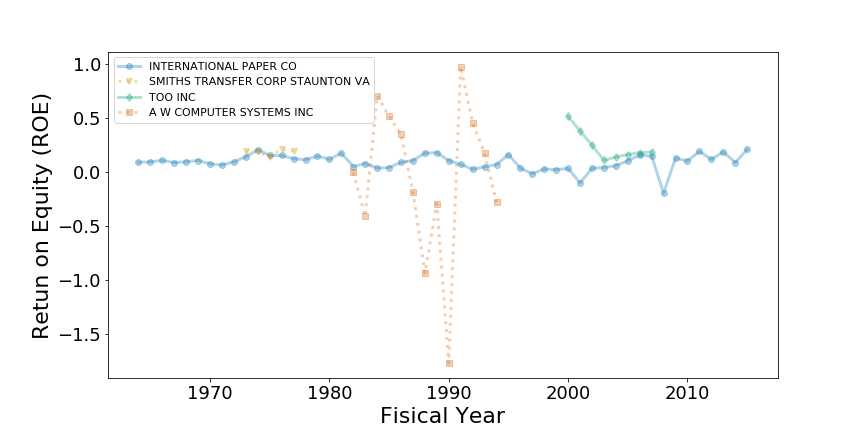
\includegraphics[width=\textwidth,height=0.87\textheight,keepaspectratio]{figures/ABIS/ABIS-DATA.png}
   \caption{This figure shows the annual return on equity (ROE) for a random selection of firms.}
      \label{fig:ABIS-DATA}
\end{sidewaysfigure*}

\begin{sidewaysfigure*}[htb!]
    \centering
    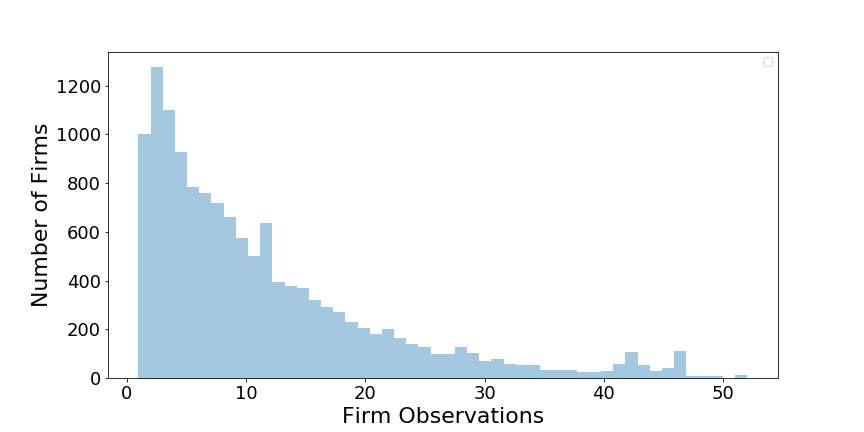
\includegraphics[width=\textwidth,height=0.87\textheight,keepaspectratio]{figures/ABIS/FirmObs.png}

   \caption{This figure shows the distribution of firm observations in our sample.}
      \label{fig:FirmObs}
\end{sidewaysfigure*}


\begin{figure*}[htb!]
    \centering
    \includegraphics[width=\textwidth,height=0.87\textheight,keepaspectratio]{figures/ABIS/analysis_1-1_ValidationCurveTrees.png}

   \caption{This figure shows validation curves for each measure in Analysis 1-1, varying the number of trees. }
      \label{fig:ValidationCurve-A1-Trees}
\end{figure*}

\begin{figure*}[htb!]
    \centering
    \includegraphics[width=\textwidth]{figures/ABIS/analysis_1-1_ValidationCurveDepth.png}

    \caption{
    		This figure shows the validation curves for each measure in Analysis 1-1 varying the max depth using  \(30\) trees in a forest. 
      }
      \label{fig:ValidationCurve-A1-Depth}
\end{figure*}

\clearpage


{\renewcommand{\arraystretch}{1.5}

\begin{table}[htb!]
\centering
\begin{tabular}{|l|l|}
\hline
\textbf{Variable}                                                          & \textbf{Code} \\ \hline
Current Assets – Total                                                     & ACT           \\ \hline
Assets – Total                                                             & AT            \\ \hline
Capital Expenditures                                                       & CAPX          \\ \hline
Common Equity – Total                                                      & CEQ           \\ \hline
Cash and Short-Term Investments                                            & CHE           \\ \hline
Debt in Current Liabilities (short-term debt)                              & DLC           \\ \hline
Long-Term Debt – Total                                                     & DLTT          \\ \hline
Depreciation and Amortization                                              & DP            \\ \hline
Data year – fiscal                                                         & FYEAR         \\ \hline
Earnings (income before extraordinary items)                               & IB            \\ \hline
Earnings (income before extraordinary items, from statement of cash flows) & IBC           \\ \hline
Interest and Related Income – Total                                        & IDIT          \\ \hline
Short-term investments – Total                                             & IVST          \\ \hline
Current Liabilities – Total                                                & LCT           \\ \hline
Liabilities – Total                                                        & LT            \\ \hline
Operating Activities – Net Cash Flow                                       & OANCF         \\ \hline
Operating Income before Depreciation                                       & OIBDP         \\ \hline
CRSP permanent number                                                      & PERMNO        \\ \hline
Property, Plant, and Equipment – Total (Net)                               & PPENT         \\ \hline
Standard Industry Classification                                           & SIC           \\ \hline
Income Taxes Payable                                                       & TXP           \\ \hline
Extraordinary Items and Discontinued Operations (Statement of Cash Flows)  & XIDOC         \\ \hline
Interest Expense                                                           & XINT          \\ \hline
\end{tabular}
\caption{Table showing the Computstat variables used in this study.}
\label{tab:CompustatVariables}
\end{table}

\begin{table}[]
\begin{tabular}{|c|c|}
\hline
Variable             & Formula                                                     \\ \hline
Net Operating Assets & $NOA_t = (AT_t - CHE_t - IVST_t) - (LT_t - DLC_t - DLTT_t)$ \\ \hline
Operating Income     & $OI_t=IB_t + XINT_t - IDIT_t$                               \\ \hline
\end{tabular}
\caption{This table shows how we compute net operating assets and operating income  by following the procedure described in \citep{LiTuna2014}. }
\label{tab:ComputstatCompute}
\end{table}

{\renewcommand{\arraystretch}{2}
\begin{table}[htb!]
\centering
\begin{tabular}{|c|c|}
\hline
\textbf{Variable} & \textbf{Definition}                           \\ \hline
$ROE_t$           & $\frac{IB_t}{0.5(CEQ_t + CEQ_{t-1})}$         \\ \hline
$ROA_t$           & $\frac{IB_t + XINT_t}{0.5(AT_t + AT_{t-1})}$    \\ \hline
$RNOA_t$          & $\frac{OI_t}{0.5 \times (NOA_t + NOA_{t-1})}$ \\ \hline
$CFO_t$           & $\frac{OANCF_t}{0.5(AT_t + AT_{t-1})}$          \\ \hline
$FCF_t$           & $\frac{OANCF_t - CAPX_t}{0.5(AT_t + AT_{t-1})}$ \\ \hline
\end{tabular}
\caption{Table showing the profitability measure definitions.}
\label{tab:ProfitMeasures} 

\end{table}


\begin{table}[htb!]
\centering
\resizebox{\columnwidth}{!}{\begin{tabular}{|l|c|c|c|c|c|c|c|c|c|c|}
\hline
\textbf{Variable} & \multicolumn{1}{l|}{\textbf{Count}} & \multicolumn{1}{l|}{\textbf{Mean}} & \multicolumn{1}{l|}{\textbf{Std}} & \multicolumn{1}{l|}{\textbf{Min}} & \multicolumn{1}{l|}{\textbf{1\%}} & \multicolumn{1}{l|}{\textbf{25\%}} & \multicolumn{1}{l|}{\textbf{50\%}} & \multicolumn{1}{l|}{\textbf{75\%}} & \multicolumn{1}{l|}{\textbf{99\%}} & \multicolumn{1}{l|}{\textbf{Max}} \\ \hline
\textbf{AT}       & 167,718.00                          & 3,344.65                           & 37,775.67                         & 0                                 & 2.08                              & 32.21                              & 139.24                             & 754.55                             & 45,009.92                          & 2,573,126.00                      \\ \hline
\textbf{CAPX}     & 167,213.00                          & 103.64                             & 665.28                            & -401.61                           & 0                                 & 0.99                               & 5.29                               & 30.46                              & 1,833.88                           & 37,985.00                         \\ \hline
\textbf{CEQ}      & 167,718.00                          & 733.70                             & 4,746.54                          & -59,640.00                        & -46.55                            & 13.94                              & 59.19                              & 272.44                             & 11,881.49                          & 255,550.00                        \\ \hline
\textbf{DP}       & 166,456.00                          & 73.70                              & 465.94                            & -7.91                             & 0.02                              & 0.95                               & 4.20                               & 23.01                              & 1,250.90                           & 22,016.00                         \\ \hline
\textbf{IB}       & 167,718.00                          & 85.78                              & 859.57                            & -99,289.00                        & -227.97                           & -0.32                              & 3.38                               & 25.86                              & 1,844.83                           & 53,394.00                         \\ \hline
\textbf{OANCF}    & 167,718.00                          & 181.91                             & 1,590.52                          & -110,560.00                       & -81.17                            & 0.10                               & 6.70                               & 51.69                              & 3,353.03                           & 129,731.00                        \\ \hline
\textbf{OIBDP}    & 167,026.00                          & 264.67                             & 1,742.21                          & -76,735.00                        & -53.35                            & 1.57                               & 13.19                              & 81.83                              & 4,516.75                           & 81,730.00                         \\ \hline
\textbf{PPENT}    & 166,826.00                          & 620.94                             & 3,822.74                          & 0                                 & 0.05                              & 4.86                               & 24.81                              & 154.47                             & 12,305.75                          & 252,668.00                        \\ \hline
\textbf{XINT}     & 167,718.00                          & 49.38                              & 639.00                            & -0.88                             & 0                                 & 0.12                               & 1.28                               & 10.41                              & 648.83                             & 57,302.00                         \\ \hline
\end{tabular}}
\caption{This table shows the descriptive statistics for the Compustat variables in the sample.}
\label{tab:CompustatDescribe}
\end{table}

\begin{table}[]
\begin{tabular}{|c|c|c|c|c|c|c|c|c|c|c|}
\hline
\textbf{Variable} & \textbf{Count} & \textbf{Mean} & \textbf{Std} & \textbf{Min} & \textbf{1\%} & \textbf{25\%} & \textbf{50\%} & \textbf{75\%} & \textbf{99\%} & \textbf{max} \\ \hline
\textbf{ROE}      & 160,653.00     & 0.00          & 0.50         & -4.47           & -2.52        & -0.01         & 0.10          & 0.17          & 1.10          & 2.97         \\ \hline
\textbf{ROA}      & 160,653.00     & 0.02          & 0.18         & -1.33           & -0.85        & 0.01          & 0.06          & 0.10          & 0.26          & 0.35         \\ \hline
\textbf{RNOA}     & 160,653.00     & 0.07          & 1.07         & -12.03          & -4.00        & 0.02          & 0.10          & 0.17          & 3.64          & 10.66        \\ \hline
\textbf{CFO}      & 160,653.00     & 0.04          & 0.16         & -0.91           & -0.68        & 0.01          & 0.07          & 0.12          & 0.34          & 0.41         \\ \hline
\textbf{FCF}      & 160,653.00     & -0.03         & 0.17         & -1.07           & -0.76        & -0.07         & 0.01          & 0.06          & 0.27          & 0.34         \\ \hline
\end{tabular}
\caption{This table shows the descriptive statistics for profitability measures.}
\label{tab:ProfitDescribe}
\end{table}


\begin{table}[htb!]
\centering
\resizebox{\columnwidth}{!}{\begin{tabular}{|c|c|c|c|c|c|}
\hline
\textbf{Fisical Year} & \textbf{ROE} & \textbf{ROA} & \textbf{RNOA} & \textbf{CFO} & \textbf{FCF} \\ \hline
2012                  & 47.6\%       & 48.4\%       & 47.9\%        & 49.4\%       & 51.9\%       \\ \hline
2013                  & 48.9\%       & 49.7\%       & 47.6\%        & 43.3\%       & 42.5\%       \\ \hline
2014                  & 46.6\%       & 45.5\%       & 44.7\%        & 49.1\%       & 51.5\%       \\ \hline
2015                  & 48.4\%       & 51.0\%       & 50.2\%        & 50.8\%       & 53.6\%       \\ \hline
\end{tabular}}
\caption{This table shows the percentage increases of annual profitability in our test sample.}
\label{tab:TargetPercentIncreases}
\end{table}


\begin{table}[htb!]
\centering
\resizebox{\columnwidth}{!}{\begin{tabular}{|c|c|c|c|c|c|c|}
\hline
\textbf{}               & \textbf{ROE} & \textbf{Ind ROE Mean} & \textbf{Ind ROE Median} & \textbf{Ind ROE Std} & \textbf{ROE\_L1} & \textbf{ROE\_L2} \\ \hline
\textbf{ROE}            & 1.00         & 0.20                  & 0.39                    & -0.11                & 0.53             & 0.39             \\ \hline
\textbf{Ind ROE Mean}   &              & 1.00                  & 0.35                    & -0.63                & 0.14             & 0.12             \\ \hline
\textbf{Ind ROE Median} &              &                       & 1.00                    & -0.19                & 0.33             & 0.29             \\ \hline
\textbf{Ind ROE Std}    &              &                       &                         & 1.00                 & -0.12            & -0.10            \\ \hline
\textbf{ROE\_L1}        &              &                       &                         &                      &                  & 0.54             \\ \hline
\textbf{ROE\_L2}        &              &                       &                         &                      &                  & 1.00             \\ \hline
\end{tabular}}
\caption{This table shows the Pearson correlations for ROE features in our sample.}
\label{tab:ROECorr}
\end{table}


\begin{table}[htb!]
\centering
\resizebox{\columnwidth}{!}{\begin{tabular}{|l|l|l|l|l|l|l|}
\hline
\textbf{}               & \textbf{ROA} & \textbf{Ind ROA Mean} & \textbf{Ind ROA Median} & \textbf{Ind ROA Std} & \textbf{ROA\_L1} & \textbf{ROA\_L2} \\ \hline
\textbf{ROA}            & 1.00         & 0.53                  & 0.49                    & -0.42                & 0.74             & 0.63             \\ \hline
\textbf{Ind ROA Mean}   &              & 1.00                  & 0.89                    & -0.84                & 0.48             & 0.43             \\ \hline
\textbf{Ind ROA Median} & \textbf{}    &                       & 1.00                    & -0.60                & 0.45             & 0.42             \\ \hline
\textbf{Ind ROA Std}    &              &                       &                         & 1.00                 & -0.38            & -0.36            \\ \hline
\textbf{ROA\_L1}        &              &                       &                         &                      & 1.00             & 0.74             \\ \hline
\textbf{ROA\_L2}        &              &                       &                         &                      &                  & 1.00             \\ \hline
\end{tabular}}
\caption{This table shows the Pearson correlations for ROA features in our sample.}
\label{tab:ROACorr}
\end{table}

\begin{table}[htb!]
\centering
\resizebox{\columnwidth}{!}{
\begin{tabular}{|l|l|l|l|l|l|l|}
\hline
\textbf{}                & \textbf{RNOA} & \textbf{Ind RNOA Mean} & \textbf{Ind RNOA Median} & \textbf{Ind RNOA Std} & \textbf{RNOA\_L1} & \textbf{RNOA\_L2} \\ \hline
\textbf{RNOA}            & 1.00          & 0.10                   & 0.24                     & 0.01                  & 0.36              & 0.22              \\ \hline
\textbf{Ind RNOA Mean}   &               & 1.00                   & 0.25                     & 0.26                  & 0.06              & 0.03              \\ \hline
\textbf{Ind RNOA Median} & \textbf{}     &                        & 1.00                     & 0.09                  & 0.18              & 0.14              \\ \hline
\textbf{Ind RNOA Std}    &               &                        &                          & 1.00                  & 0.01              & 0.01              \\ \hline
\textbf{RNOA\_L1}        &               &                        &                          &                       & 1.00              & 0.36              \\ \hline
\textbf{RNOA\_L2}        &               &                        &                          &                       &                   & 1.00              \\ \hline
\end{tabular}}
\caption{This table shows the Pearson correlations for RNOA features in our sample.}
\label{tab:RNOACorr}
\end{table}

\begin{table}[htb!]
\centering
\resizebox{\columnwidth}{!}{
\begin{tabular}{|l|l|l|l|l|l|l|}
\hline
\textbf{}               & \textbf{FCF} & \textbf{Ind FCF Mean} & \textbf{Ind FCF Median} & \textbf{Ind FCF Std} & \textbf{FCF\_L1} & \textbf{FCF\_L2} \\ \hline
\textbf{FCF}            & 1.00         & 0.49                  & 0.45                    & -0.31                & 0.62             & 0.53             \\ \hline
\textbf{Ind FCF Mean}   &              & 1.00                  & 0.89                    & -0.71                & 0.39             & 0.36             \\ \hline
\textbf{Ind FCF Median} & \textbf{}    &                       & 1.00                    & -0.46                & 0.37             & 0.33             \\ \hline
\textbf{Ind FCF Std}    &              &                       &                         & 1.00                 & -0.28            & -0.26            \\ \hline
\textbf{FCF\_L1}        &              &                       &                         &                      & 1.00             & 0.61             \\ \hline
\textbf{FCF\_L2}        &              &                       &                         &                      &                  & 1.00             \\ \hline
\end{tabular}}
\caption{This table shows the Pearson correlations for FCF features in our sample.}
\label{tab:FCFCorr}
\end{table}

\begin{table}[htb!]
\centering
\resizebox{\columnwidth}{!}{
\begin{tabular}{|l|l|l|l|l|l|l|}
\hline
\textbf{}               & \textbf{CFO} & \textbf{Ind CFO Mean} & \textbf{Ind CFO Median} & \textbf{Ind CFO Std} & \textbf{CFO\_L1} & \textbf{CFO\_L2} \\ \hline
\textbf{CFO}            & 1.00         & 0.50                  & 0.47                    & -0.32                & 0.67             & 0.60             \\ \hline
\textbf{Ind CFO Mean}   &              & 1.00                  & 0.90                    & -0.70                & 0.42             & 0.40             \\ \hline
\textbf{Ind CFO Median} & \textbf{}    &                       & 1.00                    & -0.47                & 0.40             & 0.38             \\ \hline
\textbf{Ind CFO Std}    &              &                       &                         & 1.00                 & -0.29            & -0.28            \\ \hline
\textbf{CFO\_L1}        &              &                       &                         &                      & 1.00             & 0.66             \\ \hline
\textbf{CFO\_L2}        &              &                       &                         &                      &                  & 1.00             \\ \hline
\end{tabular}}
\caption{This table shows the Pearson correlations for CFO features in our sample.}
\label{tab:CFOCorr}
\end{table}

%\begin{table}[htb!]
%\centering
%\begin{tabular}{|l|l|l|}
%\hline
 %    & 1 Lag & 2 Lags \\ \hline
%ROE  & 0.16  & 0.15   \\ \hline
%ROA  & 0.28  & 0.27   \\ \hline
%RNOA & 0.06  & 0.04   \\ \hline
%FCF  & 0.22  & 0.21   \\ \hline
%CFO  & 0.23  & 0.23   \\ \hline
%\end{tabular}
%\caption{This table shows the Autocorrelations in profitability measures.}
%\label{tab:AutCorrProfitability}
%\end{table}

\begin{table}[htb!]
\centering
\begin{tabular}{|c|c|c|c|}
\hline
\textbf{\begin{tabular}[c]{@{}c@{}}Analysis\\ (Degree of Winsorization)\end{tabular}} & \textbf{\begin{tabular}[c]{@{}c@{}}1-1 \\ (None)\end{tabular}} & \textbf{\begin{tabular}[c]{@{}c@{}}1-2 \\ (1\% per side)\end{tabular}} & \textbf{\begin{tabular}[c]{@{}c@{}}1-3 \\ (2.5\% per side)\end{tabular}} \\ \hline
ROE                                & 3          & 2                  & 3                    \\ \hline
ROA                                & 2          & 2                  & 2                    \\ \hline
RNOA                               & 4          & 2                  & 4                    \\ \hline
CFO                                & 2          & 2                  & 2                    \\ \hline
FCF                                & 2          & 2                  & 2                    \\ \hline
\end{tabular}
\caption{This table shows the maximum depth selected for each analysis and measure combination with \(B=30\).}
\label{tab:MaxDepthA1}
\end{table}



\begin{table}[htb]
\centering
\begin{tabular}{cccc}
\multicolumn{1}{l}{}                                 & \multicolumn{3}{c}{\textbf{Return on Equity (ROE)}}                                                                                              \\ \cline{2-4} 
\multicolumn{1}{c|}{}                                & \multicolumn{3}{c|}{\textbf{Analysis (Degree of Winsorization)}}                                                                                 \\ \cline{2-4} 
\multicolumn{1}{c|}{}                                & \multicolumn{1}{c|}{\textbf{1-1 (None)}} & \multicolumn{1}{c|}{\textbf{1-2 (1\% per side)}} & \multicolumn{1}{c|}{\textbf{1-3 (2.5\% per side)}} \\ \hline
\multicolumn{1}{|c|}{Mean Training Accuracy}         & \multicolumn{1}{c|}{61.1\%}              & \multicolumn{1}{c|}{61.4\%}                      & \multicolumn{1}{c|}{61.1\%}                        \\ \hline
\multicolumn{1}{|c|}{Mean Cross Validation Accuracy} & \multicolumn{1}{c|}{55.5\%}              & \multicolumn{1}{c|}{58.5\%}                      & \multicolumn{1}{c|}{55.5\%}                        \\ \hline
\multicolumn{1}{|c|}{Mean Testing Accuracy}          & \multicolumn{1}{c|}{55.2\%}              & \multicolumn{1}{c|}{56.8\%}                      & \multicolumn{1}{c|}{55.2\%}                        \\ \hline
\multicolumn{1}{|c|}{Random Walk 1}                  & \multicolumn{3}{c|}{50\%}                                                                                                                         \\ \hline
\multicolumn{1}{|c|}{Random Walk 2}                  & \multicolumn{3}{c|}{48\%}                                                                                                                    \\ \hline
\multicolumn{4}{|c|}{\textbf{Test Scores by Year}}                                                                                                                                                      \\ \hline
\multicolumn{1}{|c|}{2012}                           & \multicolumn{1}{c|}{57.5\%}              & \multicolumn{1}{c|}{60.4\%}                      & \multicolumn{1}{c|}{57.5\%}                        \\ \hline
\multicolumn{1}{|c|}{2013}                           & \multicolumn{1}{c|}{53.8\%}              & \multicolumn{1}{c|}{57.1\%}                      & \multicolumn{1}{c|}{53.8\%}                        \\ \hline
\multicolumn{1}{|c|}{2014}                           & \multicolumn{1}{c|}{55.2\%}              & \multicolumn{1}{c|}{54.2\%}                      & \multicolumn{1}{c|}{55.2\%}                        \\ \hline
\multicolumn{1}{|c|}{2015}                           & \multicolumn{1}{c|}{54.1\%}              & \multicolumn{1}{c|}{55.4\%}                      & \multicolumn{1}{c|}{54.1\%}                        \\ \hline
\multicolumn{4}{|c|}{\textbf{Feature Importance}}                                                                                                                                                       \\ \hline
\multicolumn{1}{|c|}{PERMNO}                         & \multicolumn{1}{c|}{2.7\%}            & \multicolumn{1}{c|}{2.7\%}                    & \multicolumn{1}{c|}{2.7\%}                      \\ \hline
\multicolumn{1}{|c|}{Fisical Year}                   & \multicolumn{1}{c|}{19\%}            & \multicolumn{1}{c|}{30\%}                    & \multicolumn{1}{c|}{19\%}                      \\ \hline
\multicolumn{1}{|c|}{ROE}                            & \multicolumn{1}{c|}{78.2\%}            & \multicolumn{1}{c|}{67.2\%}                    & \multicolumn{1}{c|}{78.2\%}                      \\ \hline
\end{tabular}
\caption{This table shows the results of analyses 1-1, 1-2, and 1-3 results for the profitability measure ROE.}
\label{tab:ROE-1}
\end{table}


\begin{table}[htb]
\centering
\begin{tabular}{cccc}
\textbf{}                                            & \multicolumn{3}{c}{\textbf{Return on Equity (ROA)}}                                                                                              \\ \cline{2-4} 
\multicolumn{1}{c|}{}                                & \multicolumn{3}{c|}{\textbf{Analysis (Degree of Winsorization)}}                                                                                 \\ \cline{2-4} 
\multicolumn{1}{c|}{}                                & \multicolumn{1}{c|}{\textbf{1-1 (None)}} & \multicolumn{1}{c|}{\textbf{1-2 (1\% per side)}} & \multicolumn{1}{c|}{\textbf{1-3 (2.5\% per side)}} \\ \hline
\multicolumn{1}{|c|}{Mean Training Accuracy}         & \multicolumn{1}{c|}{61.1\%}              & \multicolumn{1}{c|}{61.2\%}                      & \multicolumn{1}{c|}{61.1\%}                        \\ \hline
\multicolumn{1}{|c|}{Mean Cross Validation Accuracy} & \multicolumn{1}{c|}{57.9\%}              & \multicolumn{1}{c|}{58.1\%}                      & \multicolumn{1}{c|}{57.9\%}                        \\ \hline
\multicolumn{1}{|c|}{Mean Testing Accuracy}          & \multicolumn{1}{c|}{58.5\%}              & \multicolumn{1}{c|}{58.5\%}                      & \multicolumn{1}{c|}{58.5\%}                        \\ \hline
\multicolumn{1}{|c|}{Random Walk 1}                  & \multicolumn{3}{c|}{50\%}                                                                                                                        \\ \hline
\multicolumn{1}{|c|}{Random Walk 2}                  & \multicolumn{3}{c|}{48.1\%}                                                                                                                      \\ \hline
\multicolumn{4}{|c|}{\textbf{Test Scores by Year}}                                                                                                                                                      \\ \hline
\multicolumn{1}{|c|}{2012}                           & \multicolumn{1}{c|}{60.6\%}              & \multicolumn{1}{c|}{60.4\%}                      & \multicolumn{1}{c|}{60.6\%}                        \\ \hline
\multicolumn{1}{|c|}{2013}                           & \multicolumn{1}{c|}{57.6\%}              & \multicolumn{1}{c|}{58.2\%}                      & \multicolumn{1}{c|}{57.6\%}                        \\ \hline
\multicolumn{1}{|c|}{2014}                           & \multicolumn{1}{c|}{58.9\%}              & \multicolumn{1}{c|}{58\%}                        & \multicolumn{1}{c|}{58.9\%}                        \\ \hline
\multicolumn{1}{|c|}{2015}                           & \multicolumn{1}{c|}{56.8\%}              & \multicolumn{1}{c|}{57.2\%}                      & \multicolumn{1}{c|}{56.8\%}                        \\ \hline
\multicolumn{4}{|c|}{\textbf{Feature Importance}}                                                                                                                                                       \\ \hline
\multicolumn{1}{|c|}{PERMNO}                         & \multicolumn{1}{c|}{2.6\%}               & \multicolumn{1}{c|}{2.5\%}                       & \multicolumn{1}{c|}{2.6\%}                         \\ \hline
\multicolumn{1}{|c|}{Fisical Year}                   & \multicolumn{1}{c|}{32.2\%}              & \multicolumn{1}{c|}{32.2\%}                      & \multicolumn{1}{c|}{32.2\%}                        \\ \hline
\multicolumn{1}{|c|}{ROA}                            & \multicolumn{1}{c|}{65.2\%}              & \multicolumn{1}{c|}{65.2\%}                      & \multicolumn{1}{c|}{65.2\%}                        \\ \hline
\end{tabular}
\caption{This table shows the results of analyses 1-1, 1-2, and 1-3 results for the profitability measure ROA.}
\label{tab:ROA-1}
\end{table}


\begin{table}[htb]
\centering
\begin{tabular}{clll}
\textbf{}                                            & \multicolumn{3}{c}{\textbf{Return on Net Operating Assets (RNOA)}}                                                                               \\ \cline{2-4} 
\multicolumn{1}{c|}{}                                & \multicolumn{3}{c|}{\textbf{Analysis (Degree of Winsorization)}}                                                                                 \\ \cline{2-4} 
\multicolumn{1}{c|}{}                                & \multicolumn{1}{c|}{\textbf{1-1 (None)}} & \multicolumn{1}{c|}{\textbf{1-2 (1\% per side)}} & \multicolumn{1}{c|}{\textbf{1-3 (2.5\% per side)}} \\ \hline
\multicolumn{1}{|c|}{Mean Training Accuracy}         & \multicolumn{1}{l|}{61.2\%}              & \multicolumn{1}{l|}{62.2\%}                      & \multicolumn{1}{l|}{61.2\%}                        \\ \hline
\multicolumn{1}{|c|}{Mean Cross Validation Accuracy} & \multicolumn{1}{l|}{56.5\%}              & \multicolumn{1}{l|}{59.8\%}                      & \multicolumn{1}{l|}{56.5\%}                        \\ \hline
\multicolumn{1}{|c|}{Mean Testing Accuracy}          & \multicolumn{1}{l|}{54.1\%}              & \multicolumn{1}{l|}{53.3\%}                      & \multicolumn{1}{l|}{54.1\%}                        \\ \hline
\multicolumn{1}{|c|}{Random Walk 1}                  & \multicolumn{3}{c|}{50\%}                                                                                                                        \\ \hline
\multicolumn{1}{|c|}{Random Walk 2}                  & \multicolumn{3}{c|}{47.6\%}                                                                                                                      \\ \hline
\multicolumn{4}{|c|}{\textbf{Test Scores by Year}}                                                                                                                                                      \\ \hline
\multicolumn{1}{|c|}{2012}                           & \multicolumn{1}{l|}{59\%}                & \multicolumn{1}{l|}{55.6\%}                      & \multicolumn{1}{l|}{59\%}                          \\ \hline
\multicolumn{1}{|c|}{2013}                           & \multicolumn{1}{l|}{50\%}                & \multicolumn{1}{l|}{53.3\%}                      & \multicolumn{1}{l|}{50\%}                          \\ \hline
\multicolumn{1}{|c|}{2014}                           & \multicolumn{1}{l|}{52.7\%}              & \multicolumn{1}{l|}{50.1\%}                      & \multicolumn{1}{l|}{53\%}                          \\ \hline
\multicolumn{1}{|c|}{2015}                           & \multicolumn{1}{l|}{54.1\%}              & \multicolumn{1}{l|}{54.3\%}                      & \multicolumn{1}{l|}{54.2\%}                        \\ \hline
\multicolumn{4}{|c|}{\textbf{Feature Importance}}                                                                                                                                                       \\ \hline
\multicolumn{1}{|c|}{PERMNO}                         & \multicolumn{1}{l|}{3.2\%}               & \multicolumn{1}{l|}{1.8\%}                       & \multicolumn{1}{l|}{3.3\%}                         \\ \hline
\multicolumn{1}{|c|}{Fisical Year}                   & \multicolumn{1}{l|}{16.2\%}              & \multicolumn{1}{l|}{28.4\%}                      & \multicolumn{1}{l|}{16.2\%}                        \\ \hline
\multicolumn{1}{|c|}{RNOA}                           & \multicolumn{1}{l|}{80.5\%}              & \multicolumn{1}{l|}{69.8\%}                      & \multicolumn{1}{l|}{80.5\%}                        \\ \hline
\end{tabular}
\caption{This table shows the results of analyses 1-1, 1-2, and 1-3 results for the profitability measure RNOA.}
\label{tab:RNOA-1}
\end{table}

\begin{table}[]
\centering
\begin{tabular}{cccc}
\textbf{}                                            & \multicolumn{3}{c}{\textbf{Cash Flow from Operations (CFO)}}                                                                                             \\ \cline{2-4} 
\multicolumn{1}{c|}{}                                & \multicolumn{3}{c|}{\textbf{Analysis (Degree of Winsorization)}}                                                                                         \\ \cline{2-4} 
\multicolumn{1}{c|}{}                                & \multicolumn{1}{c|}{\textbf{1-1 (None)}} & \multicolumn{1}{c|}{\textbf{1-2 (1\% per side)}} & \multicolumn{1}{c|}{\textbf{1-3 (2.5\% per side)}} \\ \hline
\multicolumn{1}{|c|}{Mean Training Accuracy}         & \multicolumn{1}{c|}{66.5\%}                      & \multicolumn{1}{c|}{66.5\%}                      & \multicolumn{1}{c|}{66.5\%}                        \\ \hline
\multicolumn{1}{|c|}{Mean Cross Validation Accuracy} & \multicolumn{1}{c|}{63\%}                        & \multicolumn{1}{c|}{63.1\%}                      & \multicolumn{1}{c|}{0.63\%}                        \\ \hline
\multicolumn{1}{|c|}{Mean Testing Accuracy}          & \multicolumn{1}{c|}{58.7\%}                      & \multicolumn{1}{c|}{58.5\%}                      & \multicolumn{1}{c|}{58.6\%}                        \\ \hline
\multicolumn{1}{|c|}{Random Walk 1}                  & \multicolumn{3}{c|}{50\%}                                                                                                                                \\ \hline
\multicolumn{1}{|c|}{Random Walk 2}                  & \multicolumn{3}{c|}{38.2\%}                                                                                                                              \\ \hline
\multicolumn{4}{|c|}{\textbf{Test Scores by Year}}                                                                                                                                                              \\ \hline
\multicolumn{1}{|c|}{2012}                           & \multicolumn{1}{c|}{62.5\%}                      & \multicolumn{1}{c|}{62.2\%}                      & \multicolumn{1}{c|}{62.5\%}                        \\ \hline
\multicolumn{1}{|c|}{2013}                           & \multicolumn{1}{c|}{55.2\%}                      & \multicolumn{1}{c|}{54.9\%}                      & \multicolumn{1}{c|}{55.2\%}                        \\ \hline
\multicolumn{1}{|c|}{2014}                           & \multicolumn{1}{c|}{59\%}                        & \multicolumn{1}{c|}{58.9\%}                      & \multicolumn{1}{c|}{59\%}                          \\ \hline
\multicolumn{1}{|c|}{2015}                           & \multicolumn{1}{c|}{57.9\%}                      & \multicolumn{1}{c|}{0.58\%}                      & \multicolumn{1}{c|}{57.8\%}                        \\ \hline
\multicolumn{4}{|c|}{\textbf{Feature Importance}}                                                                                                                                                               \\ \hline
\multicolumn{1}{|c|}{PERMNO}                         & \multicolumn{1}{c|}{7.6\%}                       & \multicolumn{1}{c|}{7.6\%}                       & \multicolumn{1}{c|}{7.6\%}                         \\ \hline
\multicolumn{1}{|c|}{Fisical Year}                   & \multicolumn{1}{c|}{19.6\%}                      & \multicolumn{1}{c|}{19.6\%}                      & \multicolumn{1}{c|}{19.5\%}                        \\ \hline
\multicolumn{1}{|c|}{CFO}                            & \multicolumn{1}{c|}{72.8\%}                      & \multicolumn{1}{c|}{72.8\%}                      & \multicolumn{1}{c|}{72.8\%}                        \\ \hline
\end{tabular}
\caption{This table shows the results of analyses 1-1, 1-2, and 1-3 results for the profitability measure CFO.}
\label{tab:CFO-1}
\end{table}

\begin{table}[]
\centering
\begin{tabular}{clll}
\textbf{}                                            & \multicolumn{3}{c}{\textbf{Free Cash Flow (FCF)}}                                                                                                        \\ \cline{2-4} 
\multicolumn{1}{c|}{}                                & \multicolumn{3}{c|}{\textbf{Analysis (Degree of Winsorization)}}                                                                                         \\ \cline{2-4} 
\multicolumn{1}{c|}{}                                & \multicolumn{1}{c|}{\textbf{1-1 (None)}} & \multicolumn{1}{c|}{\textbf{1-2 (1\% per side)}} & \multicolumn{1}{c|}{\textbf{1-3 (2.5\% per side)}} \\ \hline
\multicolumn{1}{|c|}{Mean Training Accuracy}         & \multicolumn{1}{l|}{68.3\%}                      & \multicolumn{1}{l|}{68.4\%}                      & \multicolumn{1}{l|}{68.3\%}                        \\ \hline
\multicolumn{1}{|c|}{Mean Cross Validation Accuracy} & \multicolumn{1}{l|}{64.7\%}                      & \multicolumn{1}{l|}{64.8\%}                      & \multicolumn{1}{l|}{64.7\%}                        \\ \hline
\multicolumn{1}{|c|}{Mean Testing Accuracy}          & \multicolumn{1}{l|}{59.1\%}                      & \multicolumn{1}{l|}{59.1\%}                      & \multicolumn{1}{l|}{59.1\%}                        \\ \hline
\multicolumn{1}{|c|}{Random Walk 1}                  & \multicolumn{3}{c|}{50\%}                                                                                                                                \\ \hline
\multicolumn{1}{|c|}{Random Walk 2}                  & \multicolumn{3}{c|}{39\%}                                                                                                                                \\ \hline
\multicolumn{4}{|c|}{\textbf{Test Scores by Year}}                                                                                                                                                              \\ \hline
\multicolumn{1}{|c|}{2012}                           & \multicolumn{1}{l|}{63.2\%}                      & \multicolumn{1}{l|}{63.2\%}                      & \multicolumn{1}{l|}{63\%}                          \\ \hline
\multicolumn{1}{|c|}{2013}                           & \multicolumn{1}{l|}{55.6\%}                      & \multicolumn{1}{l|}{55.7\%}                      & \multicolumn{1}{l|}{55.6\%}                        \\ \hline
\multicolumn{1}{|c|}{2014}                           & \multicolumn{1}{l|}{60\%}                        & \multicolumn{1}{l|}{60\%}                        & \multicolumn{1}{l|}{59.8\%}                        \\ \hline
\multicolumn{1}{|c|}{2015}                           & \multicolumn{1}{l|}{57.9\%}                      & \multicolumn{1}{l|}{57.6\%}                      & \multicolumn{1}{l|}{57.9\%}                        \\ \hline
\multicolumn{4}{|c|}{\textbf{Feature Importance}}                                                                                                                                                               \\ \hline
\multicolumn{1}{|c|}{PERMNO}                         & \multicolumn{1}{l|}{3.7\%}                       & \multicolumn{1}{l|}{3.7\%}                       & \multicolumn{1}{l|}{3.7\%}                         \\ \hline
\multicolumn{1}{|c|}{Fisical Year}                   & \multicolumn{1}{l|}{20.4\%}                      & \multicolumn{1}{l|}{20.4\%}                      & \multicolumn{1}{l|}{20.5\%}                        \\ \hline
\multicolumn{1}{|c|}{FCF}                            & \multicolumn{1}{l|}{75.8\%}                      & \multicolumn{1}{l|}{75.8\%}                      & \multicolumn{1}{l|}{75.8\%}                        \\ \hline
\end{tabular}
\caption{This table shows the results of analyses 1-1, 1-2, and 1-3 results for the profitability measure FCF.}
\label{tab:FCF-1}
\end{table}

\begin{table}[]
\centering
\resizebox{!}{.35\paperheight}{
\begin{tabular}{ccccc}
\multicolumn{1}{l}{}                      & \multicolumn{4}{c}{\textbf{Return on Equity (ROE)}}                                                                                           \\ \cline{2-5} 
\multicolumn{1}{l|}{}                     & \multicolumn{4}{c|}{\textbf{Analysis}}                                                                                                        \\ \cline{2-5} 
\multicolumn{1}{l|}{}                     & \multicolumn{1}{c|}{\textbf{2-1}} & \multicolumn{1}{c|}{\textbf{2-2}} & \multicolumn{1}{c|}{\textbf{2-3}} & \multicolumn{1}{c|}{\textbf{2-4}} \\ \hline
\multicolumn{1}{|c|}{Mean Train Accuracy}          & \multicolumn{1}{c|}{60.5\%}       & \multicolumn{1}{c|}{62.4\%}       & \multicolumn{1}{c|}{62.4\%}       & \multicolumn{1}{c|}{62.5\%}       \\ \hline
\multicolumn{1}{|c|}{Mean Cross Validation Accuracy}             & \multicolumn{1}{c|}{55.4\%}       & \multicolumn{1}{c|}{56.0\%}       & \multicolumn{1}{c|}{57.2\%}       & \multicolumn{1}{c|}{56.4\%}       \\ \hline
\multicolumn{1}{|c|}{Mean Test Accuracy}           & \multicolumn{1}{c|}{55.0\%}       & \multicolumn{1}{c|}{56.6\%}       & \multicolumn{1}{c|}{56.8\%}       & \multicolumn{1}{c|}{56.5\%}       \\ \hline
\multicolumn{1}{|c|}{Random Walk 1}       & \multicolumn{4}{c|}{50\%}                                                                                                                     \\ \hline
\multicolumn{1}{|c|}{Random Walk 2}       & \multicolumn{4}{c|}{48\%}                                                                                                                   \\ \hline
\multicolumn{5}{|c|}{\textbf{Test Scores by Year}}                                                                                                                                        \\ \hline
\multicolumn{1}{|c|}{2012}                & \multicolumn{1}{c|}{57.2\%}       & \multicolumn{1}{c|}{58.2\%}       & \multicolumn{1}{c|}{60.0\%}       & \multicolumn{1}{c|}{60.0\%}       \\ \hline
\multicolumn{1}{|c|}{2013}                & \multicolumn{1}{c|}{53.2\%}       & \multicolumn{1}{c|}{55.4\%}       & \multicolumn{1}{c|}{54.8\%}       & \multicolumn{1}{c|}{55.3\%}       \\ \hline
\multicolumn{1}{|c|}{2014}                & \multicolumn{1}{c|}{55.4\%}       & \multicolumn{1}{c|}{57.4\%}       & \multicolumn{1}{c|}{56.5\%}       & \multicolumn{1}{c|}{54.2\%}       \\ \hline
\multicolumn{1}{|c|}{2015}                & \multicolumn{1}{c|}{53.9\%}       & \multicolumn{1}{c|}{55.5\%}       & \multicolumn{1}{c|}{55.9\%}       & \multicolumn{1}{c|}{56.4\%}       \\ \hline
\multicolumn{5}{|c|}{\textbf{Feature Importance}}                                                                                                                                         \\ \hline
\multicolumn{1}{|c|}{PERMNO}              & \multicolumn{1}{c|}{10.8\%}       & \multicolumn{1}{c|}{2.8\%}        & \multicolumn{1}{c|}{2.8\%}        & \multicolumn{1}{c|}{2.1\%}        \\ \hline
\multicolumn{1}{|c|}{FYEAR}               & \multicolumn{1}{c|}{32.8\%}       & \multicolumn{1}{c|}{13.5\%}       & \multicolumn{1}{c|}{8.8\%}        & \multicolumn{1}{c|}{10.8\%}       \\ \hline
\multicolumn{1}{|c|}{$ROE$}               & \multicolumn{1}{c|}{50.1\%}       & \multicolumn{1}{c|}{68.7\%}       & \multicolumn{1}{c|}{61.1\%}       & \multicolumn{1}{c|}{52.5\%}       \\ \hline
\multicolumn{1}{|c|}{SIC}                 & \multicolumn{1}{c|}{6.3\%}        & \multicolumn{1}{c|}{1.2\%}        & \multicolumn{1}{c|}{1.0\%}        & \multicolumn{1}{c|}{1.0\%}        \\ \hline
\multicolumn{1}{|c|}{Industry ROE Mean}   & \multicolumn{1}{c|}{}             & \multicolumn{1}{c|}{5.2\%}        & \multicolumn{1}{c|}{5.0\%}        & \multicolumn{1}{c|}{4.3\%}        \\ \hline
\multicolumn{1}{|c|}{Industry ROE Median} & \multicolumn{1}{c|}{}             & \multicolumn{1}{c|}{5.3\%}        & \multicolumn{1}{c|}{3.3\%}        & \multicolumn{1}{c|}{3.0\%}        \\ \hline
\multicolumn{1}{|c|}{Industry ROE std.}   & \multicolumn{1}{c|}{}             & \multicolumn{1}{c|}{3.3\%}        & \multicolumn{1}{c|}{2.6\%}        & \multicolumn{1}{c|}{2.5\%}        \\ \hline
\multicolumn{1}{|c|}{$ROE_{t-1}$}         & \multicolumn{1}{c|}{}             & \multicolumn{1}{c|}{}             & \multicolumn{1}{c|}{15.4\%}       & \multicolumn{1}{c|}{18.7\%}       \\ \hline
\multicolumn{1}{|c|}{$ROE_{t-2}$}         & \multicolumn{1}{c|}{}             & \multicolumn{1}{c|}{}             & \multicolumn{1}{c|}{}             & \multicolumn{1}{c|}{5.4\%}        \\ \hline
\end{tabular}}
\caption{This table shows the results of analyses 2-1, 2-2, 2-3, and 2-4 for the profitability measure ROE.}
\label{tab:ROE-2}
\end{table}

\begin{table}[]
\centering
\resizebox{!}{.35\paperheight}{
\begin{tabular}{ccccc}
\multicolumn{1}{l}{}                      & \multicolumn{4}{c}{\textbf{Return on Assets (ROA)}}                                                                                           \\ \cline{2-5} 
\multicolumn{1}{l|}{}                     & \multicolumn{4}{c|}{\textbf{Analysis}}                                                                                                        \\ \cline{2-5} 
\multicolumn{1}{l|}{}                     & \multicolumn{1}{c|}{\textbf{2-1}} & \multicolumn{1}{c|}{\textbf{2-2}} & \multicolumn{1}{c|}{\textbf{2-3}} & \multicolumn{1}{c|}{\textbf{2-4}} \\ \hline
\multicolumn{1}{|c|}{Mean Training Accuracy}          & \multicolumn{1}{c|}{62.2\%}       & \multicolumn{1}{c|}{61.9\%}       & \multicolumn{1}{c|}{61.4\%}       & \multicolumn{1}{c|}{61.4\%}       \\ \hline
\multicolumn{1}{|c|}{Mean Cross Validation Accuracy}             & \multicolumn{1}{c|}{59.0\%}       & \multicolumn{1}{c|}{58.3\%}       & \multicolumn{1}{c|}{58.7\%}       & \multicolumn{1}{c|}{57.3\%}       \\ \hline
\multicolumn{1}{|c|}{Mean Testing Accuracy}           & \multicolumn{1}{c|}{58.6\%}       & \multicolumn{1}{c|}{58.1\%}       & \multicolumn{1}{c|}{58.1\%}       & \multicolumn{1}{c|}{58.3\%}       \\ \hline
\multicolumn{1}{|c|}{Random Walk 1}       & \multicolumn{4}{c|}{50\%}                                                                                                                     \\ \hline
\multicolumn{1}{|c|}{Random Walk 2}       & \multicolumn{4}{c|}{48.1\%}                                                                                                                   \\ \hline
\multicolumn{5}{|c|}{\textbf{Test Scores by Year}}                                                                                                                                        \\ \hline
\multicolumn{1}{|c|}{2012}                & \multicolumn{1}{c|}{60.8\%}       & \multicolumn{1}{c|}{60.7\%}       & \multicolumn{1}{c|}{60.4\%}       & \multicolumn{1}{c|}{60.5\%}       \\ \hline
\multicolumn{1}{|c|}{2013}                & \multicolumn{1}{c|}{58.2\%}       & \multicolumn{1}{c|}{58.5\%}       & \multicolumn{1}{c|}{57.8\%}       & \multicolumn{1}{c|}{57.7\%}       \\ \hline
\multicolumn{1}{|c|}{2014}                & \multicolumn{1}{c|}{58.5\%}       & \multicolumn{1}{c|}{57.6\%}       & \multicolumn{1}{c|}{58.3\%}       & \multicolumn{1}{c|}{58.4\%}       \\ \hline
\multicolumn{1}{|c|}{2015}                & \multicolumn{1}{c|}{56.8\%}       & \multicolumn{1}{c|}{55.7\%}       & \multicolumn{1}{c|}{55.9\%}       & \multicolumn{1}{c|}{56.8\%}       \\ \hline
\multicolumn{5}{|c|}{\textbf{Feature Importance}}                                                                                                                                         \\ \hline
\multicolumn{1}{|c|}{PERMNO}              & \multicolumn{1}{c|}{4.0\%}        & \multicolumn{1}{c|}{1.1\%}        & \multicolumn{1}{c|}{0.8\%}        & \multicolumn{1}{c|}{0.7\%}        \\ \hline
\multicolumn{1}{|c|}{FYEAR}               & \multicolumn{1}{c|}{15.9\%}       & \multicolumn{1}{c|}{13.3\%}       & \multicolumn{1}{c|}{5.0\%}        & \multicolumn{1}{c|}{7.4\%}        \\ \hline
\multicolumn{1}{|c|}{$ROA$}               & \multicolumn{1}{c|}{78.3\%}       & \multicolumn{1}{c|}{70.1\%}       & \multicolumn{1}{c|}{66.7\%}       & \multicolumn{1}{c|}{56.0\%}       \\ \hline
\multicolumn{1}{|c|}{SIC}                 & \multicolumn{1}{c|}{1.8\%}        & \multicolumn{1}{c|}{1.1\%}        & \multicolumn{1}{c|}{0.8\%}        & \multicolumn{1}{c|}{0.7\%}        \\ \hline
\multicolumn{1}{|c|}{Industry ROA Mean}   & \multicolumn{1}{c|}{}             & \multicolumn{1}{c|}{5.0\%}        & \multicolumn{1}{c|}{3.6\%}        & \multicolumn{1}{c|}{3.5\%}        \\ \hline
\multicolumn{1}{|c|}{Industry ROA Median} & \multicolumn{1}{c|}{}             & \multicolumn{1}{c|}{7.4\%}        & \multicolumn{1}{c|}{5.6\%}        & \multicolumn{1}{c|}{4.0\%}        \\ \hline
\multicolumn{1}{|c|}{Industry ROA std.}   & \multicolumn{1}{c|}{}             & \multicolumn{1}{c|}{2.1\%}        & \multicolumn{1}{c|}{1.0\%}        & \multicolumn{1}{c|}{0.8\%}        \\ \hline
\multicolumn{1}{|c|}{$ROA_{t-1}$}         & \multicolumn{1}{c|}{}             & \multicolumn{1}{c|}{}             & \multicolumn{1}{c|}{16.5\%}       & \multicolumn{1}{c|}{21.3\%}       \\ \hline
\multicolumn{1}{|c|}{$ROA_{t-2}$}         & \multicolumn{1}{c|}{}             & \multicolumn{1}{c|}{}             & \multicolumn{1}{c|}{}             & \multicolumn{1}{c|}{5.7\%}        \\ \hline
\end{tabular}}
\caption{This table shows the results of analyses 2-1, 2-2, 2-3, and 2-4 for the profitability measure ROA.}
\label{tab:ROA-2}
\end{table}

\begin{table}[]
\centering
\resizebox{!}{.35\paperheight}{
\begin{tabular}{ccccc}
\multicolumn{1}{l}{}                       & \multicolumn{4}{c}{\textbf{Return on Net Operating Assets (RNOA)}}                                                                            \\ \cline{2-5} 
\multicolumn{1}{l|}{}                      & \multicolumn{4}{c|}{\textbf{Analysis}}                                                                                                        \\ \cline{2-5} 
\multicolumn{1}{l|}{}                      & \multicolumn{1}{c|}{\textbf{2-1}} & \multicolumn{1}{c|}{\textbf{2-2}} & \multicolumn{1}{c|}{\textbf{2-3}} & \multicolumn{1}{c|}{\textbf{2-4}} \\ \hline
\multicolumn{1}{|c|}{Mean Train Accuracy}           & \multicolumn{1}{c|}{60.8\%}       & \multicolumn{1}{c|}{60.8\%}       & \multicolumn{1}{c|}{61.9\%}       & \multicolumn{1}{c|}{61.9\%}       \\ \hline
\multicolumn{1}{|c|}{Mean Cross Validation Accuracy}              & \multicolumn{1}{c|}{55.9\%}       & \multicolumn{1}{c|}{56.3\%}       & \multicolumn{1}{c|}{57.1\%}       & \multicolumn{1}{c|}{56.6\%}       \\ \hline
\multicolumn{1}{|c|}{Mean Testing Accuracy}            & \multicolumn{1}{c|}{52.4\%}       & \multicolumn{1}{c|}{52.7\%}       & \multicolumn{1}{c|}{52.5\%}       & \multicolumn{1}{c|}{52.8\%}       \\ \hline
\multicolumn{1}{|c|}{Random Walk 1}        & \multicolumn{4}{c|}{50\%}                                                                                                                     \\ \hline
\multicolumn{1}{|c|}{Random Walk 2}        & \multicolumn{4}{c|}{47.6\%}                                                                                                                   \\ \hline
\multicolumn{5}{|c|}{\textbf{Test Scores by Year}}                                                                                                                                         \\ \hline
\multicolumn{1}{|c|}{2012}                 & \multicolumn{1}{c|}{59.0\%}       & \multicolumn{1}{c|}{57.0\%}       & \multicolumn{1}{c|}{57.4\%}       & \multicolumn{1}{c|}{57.8\%}       \\ \hline
\multicolumn{1}{|c|}{2013}                 & \multicolumn{1}{c|}{49.2\%}       & \multicolumn{1}{c|}{49.8\%}       & \multicolumn{1}{c|}{52.2\%}       & \multicolumn{1}{c|}{52.1\%}       \\ \hline
\multicolumn{1}{|c|}{2014}                 & \multicolumn{1}{c|}{47.5\%}       & \multicolumn{1}{c|}{49.6\%}       & \multicolumn{1}{c|}{46.9\%}       & \multicolumn{1}{c|}{47.8\%}       \\ \hline
\multicolumn{1}{|c|}{2015}                 & \multicolumn{1}{c|}{53.8\%}       & \multicolumn{1}{c|}{54.4\%}       & \multicolumn{1}{c|}{53.5\%}       & \multicolumn{1}{c|}{53.4\%}       \\ \hline
\multicolumn{5}{|c|}{\textbf{Feature Importance}}                                                                                                                                          \\ \hline
\multicolumn{1}{|c|}{PERMNO}               & \multicolumn{1}{c|}{3.6\%}        & \multicolumn{1}{c|}{1.0\%}        & \multicolumn{1}{c|}{1.4\%}        & \multicolumn{1}{c|}{0.9\%}        \\ \hline
\multicolumn{1}{|c|}{FYEAR}                & \multicolumn{1}{c|}{15.3\%}       & \multicolumn{1}{c|}{12.2\%}       & \multicolumn{1}{c|}{6.7\%}        & \multicolumn{1}{c|}{7.8\%}        \\ \hline
\multicolumn{1}{|c|}{$RNOA$}               & \multicolumn{1}{c|}{79.6\%}       & \multicolumn{1}{c|}{63.0\%}       & \multicolumn{1}{c|}{61.7\%}       & \multicolumn{1}{c|}{56.6\%}       \\ \hline
\multicolumn{1}{|c|}{SIC}                  & \multicolumn{1}{c|}{1.5\%}        & \multicolumn{1}{c|}{0.6\%}        & \multicolumn{1}{c|}{0.9\%}        & \multicolumn{1}{c|}{0.8\%}        \\ \hline
\multicolumn{1}{|c|}{Industry RNOA Mean}   & \multicolumn{1}{c|}{}             & \multicolumn{1}{c|}{6.7\%}        & \multicolumn{1}{c|}{4.5\%}        & \multicolumn{1}{c|}{4.1\%}        \\ \hline
\multicolumn{1}{|c|}{Industry RNOA Median} & \multicolumn{1}{c|}{}             & \multicolumn{1}{c|}{14.3\%}       & \multicolumn{1}{c|}{6.2\%}        & \multicolumn{1}{c|}{6.8\%}        \\ \hline
\multicolumn{1}{|c|}{Industry RNOA std.}   & \multicolumn{1}{c|}{}             & \multicolumn{1}{c|}{2.1\%}        & \multicolumn{1}{c|}{2.7\%}        & \multicolumn{1}{c|}{2.2\%}        \\ \hline
\multicolumn{1}{|c|}{$RNOA_{t-1}$}         & \multicolumn{1}{c|}{}             & \multicolumn{1}{c|}{}             & \multicolumn{1}{c|}{15.9\%}       & \multicolumn{1}{c|}{16.2\%}       \\ \hline
\multicolumn{1}{|c|}{$RNOA_{t-2}$}         & \multicolumn{1}{c|}{}             & \multicolumn{1}{c|}{}             & \multicolumn{1}{c|}{}             & \multicolumn{1}{c|}{4.5\%}        \\ \hline
\end{tabular}}
\caption{This table shows the results of analyses 2-1, 2-2, 2-3, and 2-4  for the profitability measure RNOA.}
\label{tab:RNOA-2}
\end{table}

\begin{table}[]
\centering
\resizebox{!}{.35\paperheight}{
\begin{tabular}{cllll}
\multicolumn{1}{l}{}                                 & \multicolumn{4}{c}{\textbf{Cash Flow from Operations (CFO)}}                                                                                  \\ \cline{2-5} 
\multicolumn{1}{l|}{}                                & \multicolumn{4}{c|}{\textbf{Analysis}}                                                                                                        \\ \cline{2-5} 
\multicolumn{1}{l|}{}                                & \multicolumn{1}{c|}{\textbf{2-1}} & \multicolumn{1}{c|}{\textbf{2-2}} & \multicolumn{1}{c|}{\textbf{2-3}} & \multicolumn{1}{c|}{\textbf{2-4}} \\ \hline
\multicolumn{1}{|c|}{Mean Training Accuracy}         & \multicolumn{1}{l|}{67.5\%}       & \multicolumn{1}{l|}{67.8\%}       & \multicolumn{1}{l|}{68.8\%}       & \multicolumn{1}{l|}{69.2\%}       \\ \hline
\multicolumn{1}{|c|}{Mean Cross Validation Accuracy} & \multicolumn{1}{l|}{63.9\%}       & \multicolumn{1}{l|}{64.0\%}       & \multicolumn{1}{l|}{64.5\%}       & \multicolumn{1}{l|}{64.6\%}       \\ \hline
\multicolumn{1}{|c|}{Mean Testing Accuracy}          & \multicolumn{1}{l|}{60.2\%}       & \multicolumn{1}{l|}{59.8\%}       & \multicolumn{1}{l|}{60.2\%}       & \multicolumn{1}{l|}{60.1\%}       \\ \hline
\multicolumn{1}{|c|}{Random Walk 1}                  & \multicolumn{4}{c|}{50\%}                                                                                                                     \\ \hline
\multicolumn{1}{|c|}{Random Walk 2}                  & \multicolumn{4}{c|}{38.2\%}                                                                                                                   \\ \hline
\multicolumn{5}{|c|}{\textbf{Test Scores by Year}}                                                                                                                                                   \\ \hline
\multicolumn{1}{|c|}{2012}                           & \multicolumn{1}{l|}{62.6\%}       & \multicolumn{1}{l|}{63.2\%}       & \multicolumn{1}{l|}{64.1\%}       & \multicolumn{1}{l|}{63.2\%}       \\ \hline
\multicolumn{1}{|c|}{2013}                           & \multicolumn{1}{l|}{62.6\%}       & \multicolumn{1}{l|}{58.5\%}       & \multicolumn{1}{l|}{57.5\%}       & \multicolumn{1}{l|}{58.1\%}       \\ \hline
\multicolumn{1}{|c|}{2014}                           & \multicolumn{1}{l|}{59.0\%}       & \multicolumn{1}{l|}{60.1\%}       & \multicolumn{1}{l|}{60.4\%}       & \multicolumn{1}{l|}{60.3\%}       \\ \hline
\multicolumn{1}{|c|}{2015}                           & \multicolumn{1}{l|}{56.5\%}       & \multicolumn{1}{l|}{57.3\%}       & \multicolumn{1}{l|}{58.7\%}       & \multicolumn{1}{l|}{58.7\%}       \\ \hline
\multicolumn{5}{|c|}{\textbf{Feature Importance}}                                                                                                                                                    \\ \hline
\multicolumn{1}{|c|}{PERMNO}                         & \multicolumn{1}{l|}{2.4\%}        & \multicolumn{1}{l|}{1.6\%}        & \multicolumn{1}{l|}{1.8\%}        & \multicolumn{1}{l|}{1.4\%}        \\ \hline
\multicolumn{1}{|c|}{FYEAR}                          & \multicolumn{1}{l|}{4.9\%}        & \multicolumn{1}{l|}{3.5\%}        & \multicolumn{1}{l|}{3.2\%}        & \multicolumn{1}{l|}{2.8\%}        \\ \hline
\multicolumn{1}{|c|}{$CFO$}                          & \multicolumn{1}{l|}{91.1\%}       & \multicolumn{1}{l|}{82.1\%}       & \multicolumn{1}{l|}{75.8\%}       & \multicolumn{1}{l|}{75.4\%}       \\ \hline
\multicolumn{1}{|c|}{SIC}                            & \multicolumn{1}{l|}{1.6\%}        & \multicolumn{1}{l|}{1.7\%}        & \multicolumn{1}{l|}{1.6\%}        & \multicolumn{1}{l|}{1.4\%}        \\ \hline
\multicolumn{1}{|c|}{Industry CFO Mean}              & \multicolumn{1}{l|}{}             & \multicolumn{1}{l|}{3.8\%}        & \multicolumn{1}{l|}{4.5\%}        & \multicolumn{1}{l|}{3.7\%}        \\ \hline
\multicolumn{1}{|c|}{Industry CFO Median}            & \multicolumn{1}{l|}{}             & \multicolumn{1}{l|}{5.4\%}        & \multicolumn{1}{l|}{4.4\%}        & \multicolumn{1}{l|}{4.5\%}        \\ \hline
\multicolumn{1}{|c|}{Industry CFO std.}              & \multicolumn{1}{l|}{}             & \multicolumn{1}{l|}{1.9\%}        & \multicolumn{1}{l|}{2.1\%}        & \multicolumn{1}{l|}{1.9\%}        \\ \hline
\multicolumn{1}{|c|}{$CFO_{t-1}$}                    & \multicolumn{1}{l|}{}             & \multicolumn{1}{l|}{}             & \multicolumn{1}{l|}{6.6\%}        & \multicolumn{1}{l|}{5.1\%}        \\ \hline
\multicolumn{1}{|c|}{$CFO_{t-2}$}                    & \multicolumn{1}{l|}{}             & \multicolumn{1}{l|}{}             & \multicolumn{1}{l|}{}             & \multicolumn{1}{l|}{3.8\%}        \\ \hline
\end{tabular}}
\caption{This table shows the results of analyses 2-1, 2-2, 2-3, and 2-4 for the profitability measure CFO.}
\label{tab:CFO-2}
\end{table}

\begin{table}[]
\centering
\resizebox{!}{.35\paperheight}{
\begin{tabular}{cllll}
\multicolumn{1}{l}{}                                 & \multicolumn{4}{c}{\textbf{Free Cash Flow (FCF)}}                                                                                             \\ \cline{2-5} 
\multicolumn{1}{l|}{}                                & \multicolumn{4}{c|}{\textbf{Analysis}}                                                                                                        \\ \cline{2-5} 
\multicolumn{1}{l|}{}                                & \multicolumn{1}{c|}{\textbf{2-1}} & \multicolumn{1}{c|}{\textbf{2-2}} & \multicolumn{1}{c|}{\textbf{2-3}} & \multicolumn{1}{c|}{\textbf{2-4}} \\ \hline
\multicolumn{1}{|c|}{Mean Training Accuracy}         & \multicolumn{1}{l|}{69.2\%}       & \multicolumn{1}{l|}{69.5\%}       & \multicolumn{1}{l|}{69.5\%}       & \multicolumn{1}{l|}{69.6\%}       \\ \hline
\multicolumn{1}{|c|}{Mean Cross Validation Accuracy} & \multicolumn{1}{l|}{65.2\%}       & \multicolumn{1}{l|}{65.2\%}       & \multicolumn{1}{l|}{65.5\%}       & \multicolumn{1}{l|}{65.4\%}       \\ \hline
\multicolumn{1}{|c|}{Mean Testing Accuracy}          & \multicolumn{1}{l|}{60.8\%}       & \multicolumn{1}{l|}{60.7\%}       & \multicolumn{1}{l|}{61.3\%}       & \multicolumn{1}{l|}{61.7\%}       \\ \hline
\multicolumn{1}{|c|}{Random Walk 1}                  & \multicolumn{4}{c|}{50\%}                                                                                                                     \\ \hline
\multicolumn{1}{|c|}{Random Walk 2}                  & \multicolumn{4}{c|}{39\%}                                                                                                                     \\ \hline
\multicolumn{5}{|c|}{\textbf{Test Scores by Year}}                                                                                                                                                   \\ \hline
\multicolumn{1}{|c|}{2012}                           & \multicolumn{1}{l|}{62.3\%}       & \multicolumn{1}{l|}{64.1\%}       & \multicolumn{1}{l|}{62.2\%}       & \multicolumn{1}{l|}{63.9\%}       \\ \hline
\multicolumn{1}{|c|}{2013}                           & \multicolumn{1}{l|}{63.4\%}       & \multicolumn{1}{l|}{60.4\%}       & \multicolumn{1}{l|}{63.9\%}       & \multicolumn{1}{l|}{63.3\%}       \\ \hline
\multicolumn{1}{|c|}{2014}                           & \multicolumn{1}{l|}{60.6\%}       & \multicolumn{1}{l|}{60.6\%}       & \multicolumn{1}{l|}{61.1\%}       & \multicolumn{1}{l|}{61.5\%}       \\ \hline
\multicolumn{1}{|c|}{2015}                           & \multicolumn{1}{l|}{56.9\%}       & \multicolumn{1}{l|}{57.8\%}       & \multicolumn{1}{l|}{57.9\%}       & \multicolumn{1}{l|}{58.2\%}       \\ \hline
\multicolumn{5}{|c|}{\textbf{Feature Importance}}                                                                                                                                                    \\ \hline
\multicolumn{1}{|c|}{PERMNO}                         & \multicolumn{1}{l|}{2.1\%}        & \multicolumn{1}{l|}{1.0\%}        & \multicolumn{1}{l|}{1.0\%}        & \multicolumn{1}{l|}{0.9\%}        \\ \hline
\multicolumn{1}{|c|}{FYEAR}                          & \multicolumn{1}{l|}{5.0\%}        & \multicolumn{1}{l|}{4.1\%}        & \multicolumn{1}{l|}{2.5\%}        & \multicolumn{1}{l|}{2.4\%}        \\ \hline
\multicolumn{1}{|c|}{$FCF$}                          & \multicolumn{1}{l|}{91.5\%}       & \multicolumn{1}{l|}{82.1\%}       & \multicolumn{1}{l|}{82.2\%}       & \multicolumn{1}{l|}{81.1\%}       \\ \hline
\multicolumn{1}{|c|}{SIC}                            & \multicolumn{1}{l|}{1.3\%}        & \multicolumn{1}{l|}{1.1\%}        & \multicolumn{1}{l|}{1.0\%}        & \multicolumn{1}{l|}{0.8\%}        \\ \hline
\multicolumn{1}{|c|}{Industry FCF Mean}              & \multicolumn{1}{l|}{}             & \multicolumn{1}{l|}{3.9\%}        & \multicolumn{1}{l|}{4.4\%}        & \multicolumn{1}{l|}{2.8\%}        \\ \hline
\multicolumn{1}{|c|}{Industry FCF Median}            & \multicolumn{1}{l|}{}             & \multicolumn{1}{l|}{6.0\%}        & \multicolumn{1}{l|}{3.8\%}        & \multicolumn{1}{l|}{5.0\%}        \\ \hline
\multicolumn{1}{|c|}{Industry FCF std.}              & \multicolumn{1}{l|}{}             & \multicolumn{1}{l|}{1.9\%}        & \multicolumn{1}{l|}{1.6\%}        & \multicolumn{1}{l|}{1.6\%}        \\ \hline
\multicolumn{1}{|c|}{$FCF_{t-1}$}                    & \multicolumn{1}{l|}{}             & \multicolumn{1}{l|}{}             & \multicolumn{1}{l|}{3.6\%}        & \multicolumn{1}{l|}{3.2\%}        \\ \hline
\multicolumn{1}{|c|}{$FCF_{t-2}$}                    & \multicolumn{1}{l|}{}             & \multicolumn{1}{l|}{}             & \multicolumn{1}{l|}{}             & \multicolumn{1}{l|}{2.1\%}        \\ \hline
\end{tabular}}
\caption{This table shows the results of analyses 2-1, 2-2, 2-3, and 2-4 results for the profitability measure FCF.}
\label{tab:FCF-2}
\end{table}

%\clearpage
%\bibliographystyle{plainnat}
%\bibliography{thesisbib}

\bibliographystyle{plainnat}
\nobibliography{thesisbib}